%!TeX program = lualatex
\renewcommand{\thelektion}{L12 \textperiodcentered{} Betriebssystem \& Software-Schichten}

\begin{frame}\lessontitle{Lektion 12}{Betriebssystem \& Software-Schichten}{Vom Tastendruck bis zum Bildschirm \textperiodcentered{} Skript, Kapitel 6}\end{frame}

\begin{frame}\FDUtitle{Das Problem der Komplexität}
\begin{center}
Ein Computer besteht aus vielen unterschiedlichen Hardwarekomponenten -- Prozessor, RAM, Grafikkarte, Tastatur, \ldots
\vspace{4mm}

Sollte jedes Programm direkt mit all dieser Hardware kommunizieren müssen?
\end{center}
\only<2->{\begin{center}\color{FDUteal}\bfseries Nein -- dafür gibt es das \textbf{Betriebssystem}.\end{center}}
\end{frame}

\begin{frame}\FDUtitle{Der Software-Stack}
\begin{center}
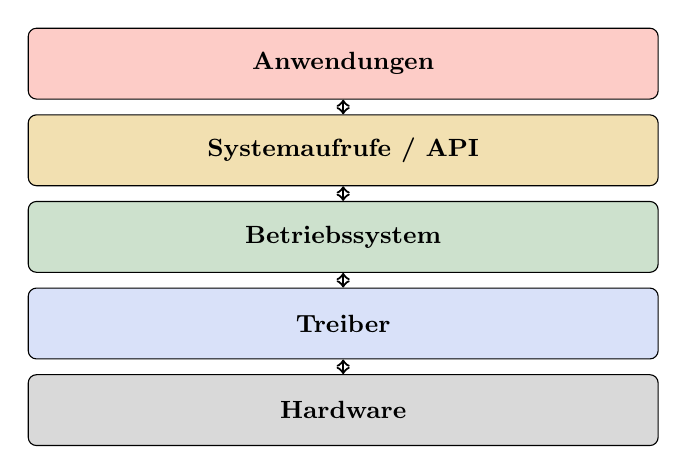
\begin{tikzpicture}[
    layer/.style={draw, minimum width=8cm, minimum height=0.9cm, text centered, rounded corners=3pt, font=\small},
]
    \node[layer, fill=Salmon!40]        (app)  at (0, 3.0) {\textbf{Anwendungen}};
    \node[layer, fill=Goldenrod!35]     (api)  at (0, 1.9) {\textbf{Systemaufrufe / API}};
    \node[layer, fill=DarkSeaGreen!45]  (os)   at (0, 0.8) {\textbf{Betriebssystem}};
    \node[layer, fill=RoyalBlue!20]     (drv)  at (0,-0.3) {\textbf{Treiber}};
    \node[layer, fill=Gray!30]          (hw)   at (0,-1.4) {\textbf{Hardware}};

    \draw[<->, thick] (app) -- (api);
    \draw[<->, thick] (api) -- (os);
    \draw[<->, thick] (os)  -- (drv);
    \draw[<->, thick] (drv) -- (hw);
\end{tikzpicture}

\end{center}
\begin{center}Jede Schicht abstrahiert die Komplexität der Ebene darunter.\end{center}
\end{frame}

\begin{frame}\FDUtitle{Abstraktion als roter Faden}
\begin{itemize}[<+->]\setlength\itemsep{6pt}
  \item Ein Byte abstrahiert von einzelnen Bits (Lektion 4)
  \item Ein Gatter abstrahiert von einzelnen Transistoren (Lektion 8)
  \item Der Software-Stack abstrahiert von der konkreten Hardware
\end{itemize}
\vspace{3mm}
\begin{center}\color{FDUteal}\bfseries Jede Schicht der Informatik baut auf einer einfacheren darunterliegenden Schicht auf.\end{center}
\end{frame}

\begin{frame}\FDUtitle{Übung: Zuordnung zum Software-Stack}
\aufgabebox{Fünf Elemente (A--E) der passenden Schicht im Software-Stack zuordnen:}
\vspace{1mm}
\begin{center}
\resizebox{0.92\textwidth}{!}{%
\begin{tikzpicture}[
    layer/.style={
        draw=#1!80!black,
        fill=#1!20,
        thick,
        minimum width=4.8cm,
        minimum height=0.72cm,
        inner ysep=4pt,
        align=center,
        rounded corners=3pt,
        font=\footnotesize
    },
    itembox/.style={
        draw=black!60,
        fill=white,
        dashed,
        thick,
        minimum width=5.4cm,
        minimum height=0.72cm,
        inner ysep=4pt,
        align=left,
        rounded corners=3pt,
        font=\footnotesize
    },
    >=stealth
]
    % Software stack layers (left, pitch 1.15cm)
    \node[layer=Salmon]         (app) at (0, 4.60) {\textbf{\faLaptop\hspace{1.5mm}Anwendungen}};
    \node[layer=Goldenrod]      (api) at (0, 3.45) {\textbf{\faPlug\hspace{1.5mm}Systemaufrufe / API}};
    \node[layer=DarkSeaGreen]   (os)  at (0, 2.30) {\textbf{\faCogs\hspace{1.5mm}Betriebssystem}};
    \node[layer=CornflowerBlue] (drv) at (0, 1.15) {\textbf{\faMicrochip\hspace{1.5mm}Gerätetreiber}};
    \node[layer=Gray]           (hw)  at (0, 0.00) {\textbf{\faServer\hspace{1.5mm}Hardware}};

    % Connecting arrows inside stack
    \foreach \from/\to in {app/api, api/os, os/drv, drv/hw} {
        \draw[<->, thick, draw=black!40] (\from) -- (\to);
    }

    % Items to be assigned (right, pitch 1.15cm)
    \node[itembox] (iA) at (6.0, 4.60) {\textbf{A}\hspace{2mm}NTFS-Dateisystem};
    \node[itembox] (iB) at (6.0, 3.45) {\textbf{B}\hspace{2mm}Google Chrome (Browser)};
    \node[itembox] (iC) at (6.0, 2.30) {\textbf{C}\hspace{2mm}CPU führt Maschinenbefehl aus};
    \node[itembox] (iD) at (6.0, 1.15) {\textbf{D}\hspace{2mm}Grafikkartentreiber};
    \node[itembox] (iE) at (6.0, 0.00) {\textbf{E}\hspace{2mm}Aufruf \texttt{open("datei.txt")}};

    % Column headers
    \node[above=4pt, font=\scriptsize\bfseries, text=black!70] at (0, 5.0) {Schichten};
    \node[above=4pt, font=\scriptsize\bfseries, text=black!70] at (6.0, 5.0) {Zuzuordnende Elemente};
\end{tikzpicture}
%
}
\end{center}
\end{frame}

\begin{frame}\FDUtitle{Lösung: Zuordnung zum Software-Stack}
\begin{center}
\resizebox{0.92\textwidth}{!}{%
\begin{tikzpicture}[
    layer/.style={
        draw=#1!80!black,
        fill=#1!20,
        thick,
        minimum width=4.8cm,
        minimum height=0.72cm,
        inner ysep=4pt,
        align=center,
        rounded corners=3pt,
        font=\footnotesize
    },
    itembox/.style={
        draw=#1!80!black,
        fill=#1!15,
        thick,
        minimum width=5.4cm,
        minimum height=0.72cm,
        inner ysep=4pt,
        align=left,
        rounded corners=3pt,
        font=\footnotesize
    },
    >=stealth
]
    % Software stack layers (left, pitch 1.15cm)
    \node[layer=Salmon]         (app) at (0, 4.60) {\textbf{\faLaptop\hspace{1.5mm}Anwendungen}};
    \node[layer=Goldenrod]      (api) at (0, 3.45) {\textbf{\faPlug\hspace{1.5mm}Systemaufrufe / API}};
    \node[layer=DarkSeaGreen]   (os)  at (0, 2.30) {\textbf{\faCogs\hspace{1.5mm}Betriebssystem}};
    \node[layer=CornflowerBlue] (drv) at (0, 1.15) {\textbf{\faMicrochip\hspace{1.5mm}Gerätetreiber}};
    \node[layer=Gray]           (hw)  at (0, 0.00) {\textbf{\faServer\hspace{1.5mm}Hardware}};

    % Connecting arrows inside stack
    \foreach \from/\to in {app/api, api/os, os/drv, drv/hw} {
        \draw[<->, thick, draw=black!40] (\from) -- (\to);
    }

    % Items to be assigned (right, pitch 1.15cm)
    \node[itembox=DarkSeaGreen]   (iA) at (6.0, 4.60) {\textbf{A}\hspace{2mm}NTFS-Dateisystem};
    \node[itembox=Salmon]         (iB) at (6.0, 3.45) {\textbf{B}\hspace{2mm}Google Chrome (Browser)};
    \node[itembox=Gray]           (iC) at (6.0, 2.30) {\textbf{C}\hspace{2mm}CPU führt Maschinenbefehl aus};
    \node[itembox=CornflowerBlue] (iD) at (6.0, 1.15) {\textbf{D}\hspace{2mm}Grafikkartentreiber};
    \node[itembox=Goldenrod]      (iE) at (6.0, 0.00) {\textbf{E}\hspace{2mm}Aufruf \texttt{open("datei.txt")}};

    % Assignment arrows from items to layers
    \draw[<-, thick, draw=Salmon!80!black]         (app.east) -- (iB.west);
    \draw[<-, thick, draw=Goldenrod!80!black]      (api.east) -- (iE.west);
    \draw[<-, thick, draw=DarkSeaGreen!80!black]   (os.east)  -- (iA.west);
    \draw[<-, thick, draw=CornflowerBlue!80!black] (drv.east) -- (iD.west);
    \draw[<-, thick, draw=Gray!80!black]           (hw.east)  -- (iC.west);

    % Column headers
    \node[above=4pt, font=\scriptsize\bfseries, text=black!70] at (0, 5.0) {Schichten};
    \node[above=4pt, font=\scriptsize\bfseries, text=black!70] at (6.0, 5.0) {Zugeordnete Elemente};
\end{tikzpicture}
%
}
\end{center}
\end{frame}

\begin{frame}\FDUtitle{Vier Aufgaben des Betriebssystems}
\begin{enumerate}[<+->]\setlength\itemsep{7pt}
  \item \tib{Prozessverwaltung} -- CPU-Zeit auf mehrere Programme aufteilen
  \item \tib{Speicherverwaltung} -- jedem Prozess einen eigenen RAM-Bereich zuweisen
  \item \tib{Dateisystem} -- Bits in Dateien und Verzeichnisse organisieren
  \item \tib{Geräteverwaltung} -- Treiber für Drucker, Netzwerk, Grafikkarte, \ldots
\end{enumerate}
\end{frame}

\begin{frame}\FDUtitle{Multitasking}
\begin{center}
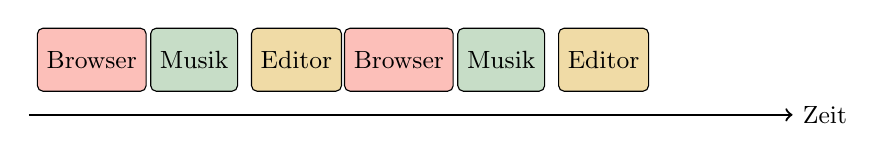
\begin{tikzpicture}[font=\small]
    \draw[thick, ->] (-0.5,0) -- (9.2,0) node[right] {Zeit};
    \foreach \x/\lbl/\col in {0/Browser/Salmon!50, 1/Musik/DarkSeaGreen!50, 2/Editor/Goldenrod!40, 3/Browser/Salmon!50, 4/Musik/DarkSeaGreen!50, 5/Editor/Goldenrod!40} {
        \node[draw, fill=\col, minimum width=1.1cm, minimum height=0.8cm, rounded corners=2pt] at (\x*1.3 + 0.3, 0.7) {\lbl};
    }
\end{tikzpicture}

\end{center}
\begin{center}
Der Prozessor wechselt so schnell zwischen Programmen (\tib{Zeitscheiben}), dass es sich für uns nach Gleichzeitigkeit anfühlt.
\end{center}
\only<2->{
\begin{center}\textbf{Übung}: 5 Programme, je 20 ms Zeitscheibe -- wann ist ein Programm wieder an der Reihe?\end{center}}
\end{frame}

\begin{frame}\FDUtitle{Speicherschutz \& Dateisystem}
\begin{columns}[T,onlytextwidth]
\begin{column}{.46\textwidth}
\large\bfseries\color{FDUteal}Speicherschutz
\vspace{2mm}
\normalsize Verhindert, dass ein Prozess in den Speicherbereich eines anderen eingreift -- erinnert an das Risiko der Von-Neumann-Architektur (Lektion 10).
\end{column}
\begin{column}{.46\textwidth}
\large\bfseries\color{FDUblue}Dateisystem
\vspace{2mm}
\normalsize Organisiert rohe Bitsequenzen auf SSD/HDD in Dateien und Verzeichnisse (z.\,B.\ NTFS, ext4, APFS).
\end{column}
\end{columns}
\end{frame}
% 
\begin{frame}\FDUtitle{Vom Tastendruck zum Bildschirm}
\begin{center}
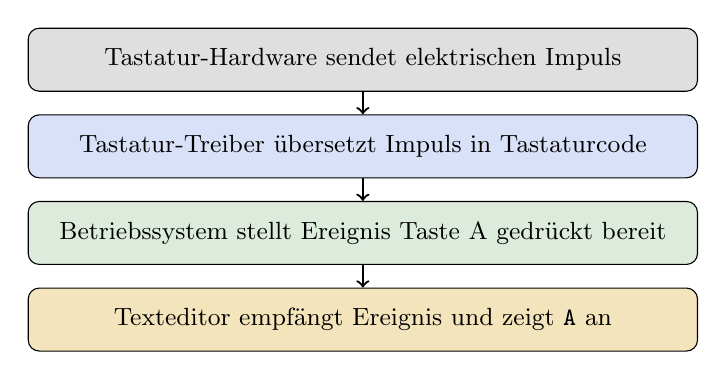
\begin{tikzpicture}[
    stepc/.style={draw, rounded corners, fill=RoyalBlue!15, minimum width=8.5cm, minimum height=0.8cm, text centered, font=\small},
    arrow/.style={->, thick}
]
    \node[stepc, fill=Gray!25]          (hw)  at (0, 3.3) {Tastatur-Hardware sendet elektrischen Impuls};
    \node[stepc, fill=RoyalBlue!20]     (drv) at (0, 2.2) {Tastatur-Treiber übersetzt Impuls in Tastaturcode};
    \node[stepc, fill=DarkSeaGreen!30]  (os)  at (0, 1.1) {Betriebssystem stellt Ereignis \enquote{Taste A gedrückt} bereit};
    \node[stepc, fill=Goldenrod!30]     (app) at (0, 0.0) {Texteditor empfängt Ereignis und zeigt \texttt{A} an};

    \draw[arrow] (hw)  -- (drv);
    \draw[arrow] (drv) -- (os);
    \draw[arrow] (os)  -- (app);
\end{tikzpicture}

\end{center}
\begin{center}Jede Schicht hat eine klar definierte Aufgabe.\end{center}
\end{frame}
% 
\begin{frame}\FDUtitle{Bekannte Betriebssysteme}
\begin{table}[H]
    \centering
    \begin{tabular}{lll}
        \textbf{OS} & \textbf{Hersteller} & \textbf{Einsatzgebiet} \\\midrule
        Windows 11 & Microsoft & PC, Laptop \\
        macOS & Apple & Mac-Computer \\
        GNU+Linux & Open Source & Server, PC, Laptop, eingebettete Systeme \\
        Android & Google & Smartphones, Tablets \\
        iOS & Apple & iPhone, iPad \\
    \end{tabular}
\end{table}
\begin{center}Über 90\,\% der Webserver laufen unter Linux -- Open-Source-Code, den jede/-r einsehen und verändern kann.\end{center}
\end{frame}
% 
\begin{frame}
\centerstatement[FDUblue]{Von der Kerbe im Ishango-Knochen bis zum Betriebssystem}{Wir haben den gesamten Weg verfolgt: Zahlendarstellung, Kodierung, logische Gatter, Computer-Hardware und Betriebssystem. Beschreiben Sie in eigenen Worten, was auf allen Ebenen passiert, wenn Sie \enquote{Strg+S} drücken.}
\end{frame}

\begin{frame}\FDUtitle{Auftrag}
\normalsize\color{FDUink!70}Skript \enquote{Aufbau und Funktionsweise eines Computers}, Kapitel 6, gesamtes Kapitel
\vspace{3mm}
\aufgabebox{\textbf{Aufgabe 6.1}: Rechendauer bei Multitasking mit 5 Prozessen}
\vspace{2mm}
\aufgabebox{\textbf{Aufgabe 6.2}: Komponenten dem Software-Stack zuordnen}
\vspace{2mm}
\challengebox{\textbf{Aufgabe 6.3}: Der ganze Weg von \enquote{Strg+S} bis zur gespeicherten Datei}
\end{frame}
